\chapter{Methodology for Analyses}
\label{chap:estimation}
In this section a brief overview of the algorithm for estimating the fatigue life of dynamic power cable will be presented. 
\section{Global Analysis}
First, the global analysis was carried out. The global model is described in Section \ref{sec:globmod} was used and the 160 sea states presented in Figure \ref{fig:scatn} was analyzed for 1 hour each, with Far weather conditions described in Section \ref{sec:current}. The following three quantities from the analyses were stored in separate files for each time step:
\begin{itemize}
    \item The  tension in the upper element of the cable.
    \item The displacement of the dummy node on the vessel in x, y and z direction.
    \item The  displacement of first and second node in the top the cable in x, y and z direction.
\end{itemize}

\subsection{Post Processing of Global Analyses Results}
The results from the global analyses determined the input of the local analysis. Time series of the displacements of the three nodes seen in Figure \ref{fig:angle} was used to calculate the angle ($\theta$) between the vessel and the cable: 

\begin{equation}
    cos(\theta) = \frac{\boldsymbol{a \cdot b}}{|\boldsymbol{a}||\boldsymbol{b}| }
\end{equation}
\begin{equation}
    cos(\theta) = \frac{a_x b_x + a_z b_z}{\sqrt{a_x^2 +a_z^2}\sqrt{b_x^2 +b_z^2}}
\end{equation}
Where $\boldsymbol{a}$ and $\boldsymbol{b}$ are the vectors of the dummy element and the first element of the cable, and $a_x$, $a_z$, $b_x$ and $b_z$ are the x and z components of the vectors $\boldsymbol{a}$ and $\boldsymbol{b}$. 

\begin{figure}[H]
\centering
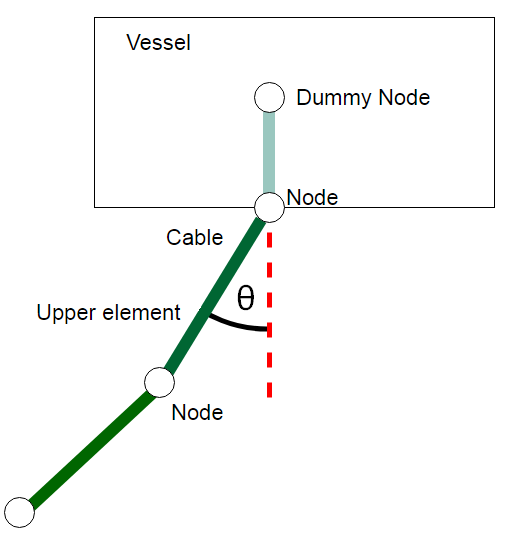
\includegraphics[scale=0.5]{figures/angle}
\caption[Angle between vessel and cable ]{Angle between vessel and cable  }
 \label{fig:angle}
\end{figure}

\noindent The calculated angle and tension were stored as time series for each sea state, and and examples of this can be seen in Figure \ref{fig:angleex} and Figure \ref{fig:extension}

\begin{figure}[H]
\subfloat[Time series for angle between vessel and cable \label{fig:angleex}]
  {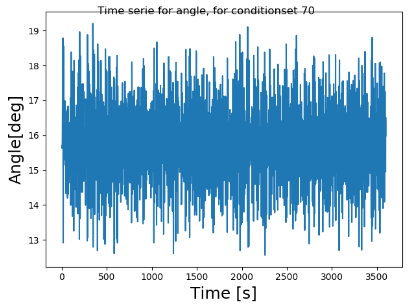
\includegraphics[width=.45\linewidth]{figures/angleex}}\hfill
\subfloat[Time series for tension in the upper element \label{fig:tensex}]
  {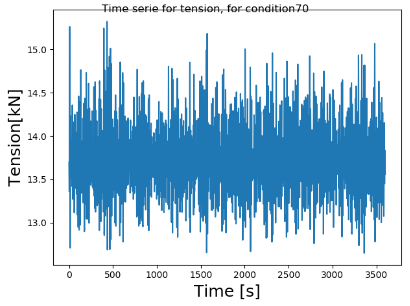
\includegraphics[width=.45\linewidth]{figures/tensex}}\hfill
\caption{Example of time series for angle and tension}
\label{fig:local1}
\end{figure}

\subsection{Rainflow Counting}
 Rainflow Counting was performed on the time series of the angle to determine the number of cycles for each angle range. The Rainflow Counting was performed in Python, and the algorithm is explained in Section \ref{sec:rainflow}. The Rainflow counting in Python gives a matrix where the first column is the class and the second is the number of cycles in each class. The counts from each sea state were scaled to apply for a year according to:

\begin{equation}
    n_{cycle,year}=n_{cycle,hour} \frac{n_{seastate}}{N_{seastate}} \cdot 365 \cdot 24 
\end{equation}

\noindent Where $n_{cycle,year}$ is the number of cycles of in an angle class in a whole year, $n_{cycle,hour}$ is the number of cycles in an angle class for an hour, calculated by the global analyses, $n_{seastate}$ is the number of observations of a certain sea state according to the scatter diagram in Figure \ref{fig:scatn} and $N_{seastate}$ is the total number of sea states in the scatter diagram in Figure \ref{fig:scatn}.\newline
\newline 
\noindent The results from the Rainflow Counting can be seen in Figure \ref{fig:initialcyc}.  

\begin{figure}[H]
\centering
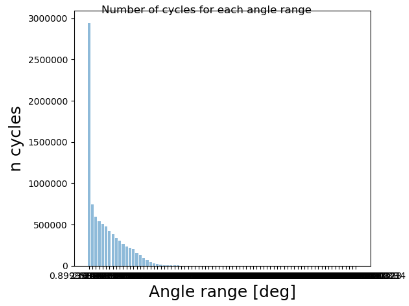
\includegraphics[scale=0.9]{figures/initialcyc}
\caption[Number of cycles in each class]{Number of cycles in each class}
 \label{fig:initialcyc}
\end{figure}

\noindent In Figure \ref{fig:initialcyc}, the classes are of equal length of 0.3. It is not possible to see the classes on the x-axis due to the large amount of classes. It is is clear from Figure \ref{fig:initialcyc} that the majority of the cycles are happening in the first classes, and decreasing as the angle increases.\newline
\newline
The damage from each cycle was calculated according to Miner Palmgren expression in Equation \ref{eq:MP}, where N was calculated from Equation \ref{eq:sn}. This gave the following expression for the damage from each angel class: 
\begin{equation}
    d_i  = \frac{n_i}{N_i}
\end{equation}
\begin{equation}
    d_i=\frac{n_i}{\frac{c}{\Delta \sigma ^m}}
\end{equation}
Where $d_i$ is the damage from the cycles in angel class i, $n_i$ is the number of cycles in angle class i, $N_i$ is the number of cycles until failure for angle class i, c is a constant from Equation \ref{eq:sn}, c=4 for this case, $\Delta \sigma$ is the stress range that relates to the angle range as: $\Delta \sigma_i = a \Delta \theta_i$ where a is an arbitrary constant.\newline
\newline 
The damage from the cycles in the different angle classes can be seen in Figure \ref{fig:initialdam}

\begin{figure}[H]
\centering
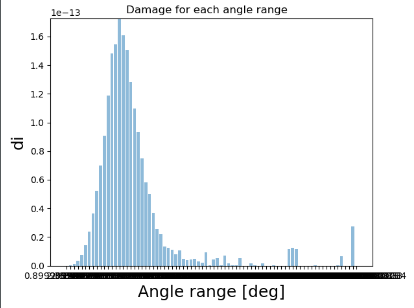
\includegraphics[scale=0.9]{figures/initialdam}
\caption[Damage for each angle class]{Damage for each angle class}
 \label{fig:initialdam}
\end{figure}
\noindent In order to get good results for the local analysis, the classes needed to be merged and rearranged so that the damage was approximately the same over each class. The results of this rearrangement can be seen in Figure \ref{fig:initialdam}

\begin{figure}[H]
\centering
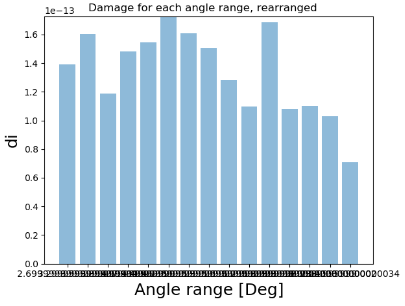
\includegraphics[scale=0.9]{figures/newdam}
\caption[Damage for each angle class, rearranged]{Damage for each angle class, rearranged}
 \label{fig:newdam}
\end{figure}

The rearrangement of the classes led to the cycle distribution shown in Figure \ref{fig:newcyc} and Table \ref{table:angleclass}:

\begin{figure}[H]
\centering
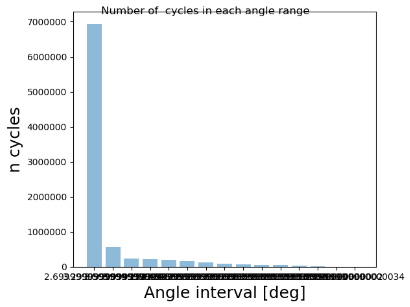
\includegraphics[scale=1]{figures/newcyc}
\caption[Distribution of cycles for each angle class, rearranged for equal damage]{Distribution of cycles for each angle class, rearranged for equal damage}
 \label{fig:newcyc}
\end{figure}

\begin{table} [H]
\centering
\begin{tabular}{ |c|c|}
\hline
Angle range class [deg] & Number of cycles \\
 \hline
 \hline
0.0 - 2.7 & 6930399.8\\

2.8 - 3.3 & 571967.9\\
 
3.4 - 3.6 & 237278.5 \\
 
3.7 - 3.9& 219492.0  \\

4.0 - 4.2& 198970.4  \\

4.3  - 4.5 & 154052.1  \\

4.6 - 4.8 & 130555.0 \\

4.9 - 5.1 & 93955.7 \\

5.2 - 5.4 & 68946.3 \\

5.5 - 5.7 & 46839.2 \\

5.8 - 6.3 & 54651.8 \\

6.4 - 6.9 & 24288.7 \\

7.0 - 8.4 & 16385.8 \\

8.5 - 18.0 & 3355.4 \\

18.1 - 23.4 & 139.3  \\

 \hline
\end{tabular}
\caption{Number of cycles in each angle range}
\label{table:angleclass}
\end{table} 
\noindent It is important to note that the number of cycles for each class are not just half and whole cycles, as the number of cycles have been scaled for occurrence during a year.\newline 
\newline

\section{Local Analysis}
The local analyses was performed by using the results from the global analyses. Each of the angle ranges was analyzed for one cycle. As the local model was pinned in both ends, both ends of the model experienced rotation when a dynamic angle was applied to the model. This can be seen in Figure \ref{fig:anglecorr}. $\theta_1$ was equal to the applied angle, but the total angle experienced by the model was:
\begin{equation}
    \theta_{tot}=\theta_1 + \theta_2
\end{equation}
Where $\theta_{tot}$ is the total angle experienced by the local model and $\theta_1$ and $\theta_2$ are illustrated in Figure \ref{fig:anglecorr}.

\begin{figure}[H]
\centering
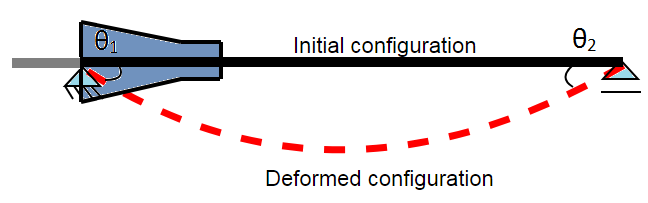
\includegraphics[scale=0.75]{figures/anglecorr}
\caption[Initial and deformed configuration of local model]{Initial and deformed configuration of local model}
 \label{fig:anglecorr}
\end{figure}

\noindent Several analyses were done to create a relation between the applied angle and the total angle. The relationship was found to be linear with a coefficient of determination ($R^2$) of 0.9978. The linear relationship can be seen in Figure \ref{fig:anglerel}, with the following expression:

\begin{equation}
    \theta_{tot}=1.2694\theta_{appl.}
\end{equation}
Where $\theta_{tot}$ is the total angle experienced by the local model and $\theta_{appl.}$ is the angle applied by BFLEX.
\begin{figure}[H]
\centering
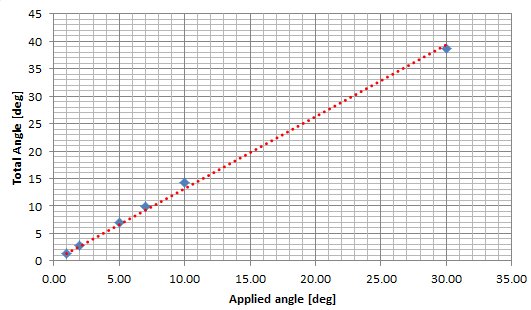
\includegraphics[scale=0.8]{figures/anglerel}
\caption[Relationship between applied angle and total angle]{Relationship between applied angle and total angle}
 \label{fig:anglerel}
\end{figure}

\noindent It was decided in line with Professor Svein Sævik's recommendations that the angle would be the master over the tension, meaning that for the local analyses, the cycle count for the angle would be used with the corresponding tension. Even though the trends in the angle time series and the tension time series were the same, the high angles and tensions did not occur at the exact same time steps, so that linear regression showed no correlation. It was decided that the max tension would correspond to the max angle, and the min angle would correspond to the min angle, as this would be a conservative approach.  Linear interpolation was used to find the tension to the corresponding angle. The max and min tension registered at the top of the cable for all sea states was 40.69 kN and 9.32 kN. \newline
\newline
\noindent The 15 angle range classes in Table \ref{table:angleclass} was turned into the 15 BFLEX cases displayed in Appendix \ref{appendix:C}. As the angles needed to be corrected due to the boundary conditions of the local model as seen in Figure \ref{fig:anglerel}, the Min angle and Max angle in Table \ref{table:loadcase} are the corrected min and max angle, and thus the angle input in the local analyses. The minimum dynamic tension and maximum dynamic tension were found through interpolation, and the mean tension represents the static tension at the top of the cable after current has been applied in far position. 





